\documentclass[11pt]{article}
\usepackage[T1]{fontenc}
\usepackage{lmodern}
\usepackage[margin=1.1in]{geometry}
\usepackage{microtype}
\usepackage{amsmath,amssymb,amsthm,mathtools}
\usepackage{graphicx}
\usepackage{booktabs}
\usepackage{enumitem}
\usepackage[dvipsnames]{xcolor}
\usepackage[colorlinks=true,linkcolor=MidnightBlue,citecolor=MidnightBlue,urlcolor=MidnightBlue]{hyperref}
\usepackage[capitalise,nameinlink]{cleveref}

\newcommand{\NexactMax}{400}
\newcommand{\SlopeCE}{-0.99}
\newcommand{\SlopeGen}{-1.00}
\newcommand{\GapGen}{1.10}
\newcommand{\NmaxCE}{131072}
\newcommand{\ErrCEmax}{2.4\times10^{-5}}
\newcommand{\FquarterLast}{0.666660}
\newcommand{\SmoothErr}{2.8\times10^{-3}}
\newcommand{\GradJump}{0.266787}
\newcommand{\GradNaive}{0.180050}
\newcommand{\GradRelErr}{32.5}
\newcommand{\FDdiff}{4.7\times10^{-10}}
\newcommand{\SlopeAdj}{-1.00}
\newcommand{\AdjointRows}{8 & 0.277037 & $1.02\times10^{-2}$ & 0.0970 \\
32 & 0.269595 & $2.81\times10^{-3}$ & 0.0895 \\
128 & 0.267505 & $7.17\times10^{-4}$ & 0.0875 \\
512 & 0.266968 & $1.80\times10^{-4}$ & 0.0869 \\
2048 & 0.266833 & $4.51\times10^{-5}$ & 0.0868 \\
8192 & 0.266799 & $1.13\times10^{-5}$ & 0.0867 \\}
\newcommand{\FixedLast}{0.0000}
\newcommand{\HalfLast}{0.6667}
\newcommand{\ThirdLast}{0.8889}
\newcommand{\NmaxFive}{65536}


\newtheorem{theorem}{Theorem}
\newtheorem{proposition}[theorem]{Proposition}
\newtheorem{lemma}[theorem]{Lemma}
\newtheorem{corollary}[theorem]{Corollary}
\theoremstyle{definition}
\newtheorem{definition}[theorem]{Definition}
\newtheorem{example}[theorem]{Example}
\theoremstyle{remark}
\newtheorem{remark}[theorem]{Remark}

\newcommand{\R}{\mathbb{R}}
\newcommand{\N}{\mathbb{N}}
\newcommand{\dd}{\,\mathrm{d}}
\newcommand{\1}{\mathbf{1}}
\newcommand{\fl}[1]{\lfloor #1\rfloor}
\newcommand{\weak}{\Rightarrow}
\DeclareMathOperator*{\esssup}{ess\,sup}

\title{\textbf{Moving spikes and measure-valued limits of backward recurrences},\\[2pt]
\large with an application to backpropagation through residual networks}
\author{Adib Alqurashi\\[2pt]
\small King Fahd University of Petroleum and Minerals, Dhahran, Saudi Arabia}
\date{\small November 2026 \quad$\cdot$\quad Principia project MathDB 354674}

\begin{document}
\maketitle

\begin{abstract}
Backward recurrences $F_n(k)=G_n(k)+H_n(k)F_n(k+1)$ appear in optimal stopping, dynamic
programming and backpropagation, and are routinely replaced by the linear differential
equation $y'=-g+hy$ built from the scaled coefficients $g_n=nG_n$ and $h_n=n(1-H_n)$.
Bay\'on, Fortuny Ayuso, Grau, Oller-Marc\'en and Ruiz conjectured that pointwise convergence
of the scaled coefficients, together with uniqueness of the admissible terminal value of the
limiting equation, forces pointwise convergence of the recurrence to the solution of that
equation. A recent counterexample, found and machine-checked in Lean on the Principia platform,
shows that a single unit spike in $G_n$ that moves with $n$ leaves a jump in the limit.
We identify the correct limit object. If $h_n\to h$ uniformly, the forcing is nonnegative,
the forcing measures $\nu_n=\sum_k G_n(k)\,\delta_{k/n}$ converge weakly to $\nu$, and the terminal
values converge, then the recurrence converges at every non-atom of $\nu$ to an explicit Duhamel
formula, the solution of the measure-driven equation $\mathrm{d}f=hf\dd x-\mathrm{d}\nu$; atoms of
$\nu$ become jumps of the same size. As corollaries, uniform integrability of $g_n$ gives
convergence to the classical solution (given convergence of the terminal values), spikes at a
fixed index wash out while spikes at a fixed relative position survive, and the limit of the
counterexample is recovered away from its jump. Numerical experiments confirm $O(1/n)$ convergence. Finally we observe
that backpropagation through a residual network is a recurrence of exactly this form, in which
intermediate losses are spikes: the continuous adjoint of the corresponding neural ODE must
jump, and dropping the jump changes a parameter gradient by $\GradRelErr\%$ in a small experiment.
\end{abstract}

\tableofcontents
\bigskip

%=====================================================================
\section{Introduction}\label{sec:intro}
%=====================================================================

Many sequential decision problems are solved by \emph{backward induction}. In the classical
secretary problem and its many variants \cite{GM66,Fer89}, the optimal expected reward from
stage $k$ onwards satisfies a recursion of the form
\begin{equation}\label{eq:rec}
F_n(k)=G_n(k)+H_n(k)\,F_n(k+1),\qquad 0\le k<n,\qquad F_n(n)=\mu,
\end{equation}
where $G_n$ is a reward collected at stage $k$ and $H_n$ is a discount or continuation
probability. To understand such problems for large $n$, Bay\'on, Fortuny Ayuso, Grau,
Oller-Marc\'en and Ruiz \cite{BFGOR23} proposed to read \eqref{eq:rec} as a discretisation
of a differential equation. Put
\begin{equation}\label{eq:scaled}
f_n(x)=F_n(\fl{nx}),\qquad g_n(x)=nG_n(\fl{nx}),\qquad h_n(x)=n\bigl(1-H_n(\fl{nx})\bigr).
\end{equation}
Then \eqref{eq:rec} reads $f_n(x)-f_n(x+\tfrac1n)=\tfrac1n\bigl(g_n(x)-h_n(x)f_n(x+\tfrac1n)\bigr)$
at the grid points, an explicit Euler step taken backward in $x$ for
\begin{equation}\label{eq:ode}
y'(x)=-g(x)+h(x)\,y(x).
\end{equation}
In \cite[Conjecture~1]{BFGOR23} they asked whether pointwise convergence of the coefficients
suffices:

\begin{quote}\itshape
If $g_n\to g$ and $h_n\to h$ pointwise on $(0,1)$ with $g,h$ continuous, and \eqref{eq:ode}
admits a solution on $(0,1]$ only for the terminal value $y(1)=\Theta$, then $f_n$ converges
pointwise on $(0,1)$ to the $C^1$ solution of \eqref{eq:ode} with $f(1)=\Theta$.
\end{quote}

The conjecture is MathDB problem 354674. It was resolved negatively on the Principia platform
\cite{Pri26}, with a Lean~4 formalisation of the decisive computations \cite{PriLean}: a single
unit spike in $G_n$, placed at the index $\fl{n/2}+1$, produces a limit with a jump of size one,
even though $g_n\to0$ pointwise and the limiting equation selects $y\equiv0$
(\cref{sec:counterexample}). The Principia solution closes with four follow-up questions:
averaged coefficient control, limits with concentrated mass, endpoint selection, and
quantitative convergence.

\paragraph{What this paper adds.} The counterexample is not an accident but an instance of a
general and simple principle: \emph{a backward recurrence does not see the values of its
forcing, it sees its mass.} Our contributions are as follows.
\begin{enumerate}[leftmargin=2em,itemsep=2pt]
\item \textbf{A measure-valued limit theorem} (\cref{thm:main}). If $h_n\to h$ uniformly and
the forcing measures $\nu_n=\sum_k G_n(k)\delta_{k/n}$ converge weakly to $\nu$, then $f_n$
converges at every non-atom of $\nu$ to
\[
f(x)=\int_{[x,b]}\Phi(x,s)\dd\nu(s)+\Theta\,\Phi(x,b),\qquad \Phi(x,s)=\exp\Bigl(-\int_x^s h\Bigr).
\]
This addresses the second follow-up question of \cite{Pri26} (limits with concentrated mass)
for the class of nonnegative forcings.
\item \textbf{Structure of the limit} (\cref{prop:structure}): $f$ is left-continuous, jumps by
exactly $\nu(\{c\})$ at each atom $c$, and solves the measure-driven equation
$\mathrm{d}f=hf\dd x-\mathrm{d}\nu$ in integral form; for $\nu=g\dd s$ with $g$ continuous it is
the solution of \eqref{eq:ode}.
\item \textbf{Convergence under uniform integrability} (\cref{cor:ui}): if $g_n\to g$ in $L^1$
(for instance pointwise and uniformly integrable), $f_n$ converges at every point to the
classical solution of \eqref{eq:ode} whose terminal value is $\lim_nF_n(K_n)$. This gives a
partial answer to the first follow-up question (averaged coefficient control), under uniform
convergence of $h_n$ and convergence of the terminal values.
\item \textbf{Fixed versus moving spikes} (\cref{cor:spikes}): a spike at a fixed index, or at
index $o(n)$, washes out; a spike at relative position $c\in(0,b)$ survives as a jump at $c$.
This explains, and recovers exactly, the counterexample.
\item \textbf{Experiments} (\cref{sec:numerics}) confirming every prediction with
$O(1/n)$ errors, including a generic test with smooth forcing, a perturbed $h_n$ and two
moving spikes.
\item \textbf{A reading of backpropagation} (\cref{sec:sciml}). Backpropagation through a
residual network \cite{E17,HR18,CRBD18} is exactly a recurrence \eqref{eq:rec} for the adjoint
$\lambda_k=\partial L/\partial z_k$. Intermediate losses, as in deep supervision or time-series
training with intermediate observations \cite{RCD19}, are moving spikes; the familiar jump
condition of the continuous adjoint is then a corollary of \cref{thm:main}, and an adjoint built
from the pointwise limits of the coefficients gives an $O(1)$ gradient error
(\cref{prop:adjoint}, \cref{tab:adjoint}).
\end{enumerate}

The proofs are elementary: a discrete Duhamel formula, a uniform estimate for products of
the form $\prod(1-h_n/n)$, and the portmanteau theorem. We include them in full because the
statements are exactly what is needed to tell, in a given application, whether a backward
recursion converges to the differential equation one has in mind.

\paragraph{Credit and related work.} The counterexample of \cref{sec:counterexample}, its exact
closed form and the Lean formalisation of its discrete computations are due to the Principia
solution \cite{Pri26,PriLean}; we reproduce them with proofs for completeness. Related failures
caused by exceptional boundary coefficients were pointed out earlier by Ravsky \cite{Rav24}, in
examples where every terminal value is admissible. Difference equations and measure differential
equations are both special cases of Kurzweil's generalized ordinary differential equations, for
which continuous-dependence theorems are available \cite{Sch92,MST19}; \cref{thm:main} should be
read as an elementary, self-contained instance for additive forcing, and we have not checked
whether it follows from those results. In \cref{sec:sciml}, the jump condition at observation
times and the consistency of discrete and continuous adjoints are standard
\cite{CRBD18,Hag00,SS16,GKB19}; what is new there is reading intermediate losses as moving spikes,
so that the jump condition becomes a corollary of \cref{thm:main}. The theorem, its consequences
and the experiments of \cref{sec:measure,sec:consequences,sec:numerics} are new to this paper.

%=====================================================================
\section{Setting and a discrete Duhamel formula}\label{sec:setting}
%=====================================================================

Throughout, $b\in(0,1]$ and $(K_n)$ are integers with
\begin{equation}\label{eq:Kn}
0<K_n\le nb,\qquad K_n/n\to b.
\end{equation}
(The original problem has $b=1$ and $K_n=n$; a terminal point $b<1$ allows equations whose
coefficient $h$ blows up at $1$, as in the counterexample.) We consider real numbers
$G_n(k),H_n(k)$ for $0\le k<K_n$, terminal values $\mu_n$, and $F_n$ defined by
\begin{equation}\label{eq:recK}
F_n(K_n)=\mu_n,\qquad F_n(k)=G_n(k)+H_n(k)F_n(k+1)\quad(0\le k<K_n).
\end{equation}
We use the scaled functions \eqref{eq:scaled} on $[0,K_n/n)$, and in addition the
\emph{forcing measure} and the \emph{discrete propagator}
\begin{equation}\label{eq:numeasure}
\nu_n=\sum_{k=0}^{K_n-1}G_n(k)\,\delta_{k/n},\qquad
P_n(k,m)=\prod_{\ell=k}^{m-1}H_n(\ell)\quad(0\le k\le m\le K_n),
\end{equation}
with the empty product equal to $1$. Note that $h_n(\ell/n)=n(1-H_n(\ell))$ exactly, and that
$\nu_n$ has the same total mass as $g_n$: $\nu_n([0,b])=\sum_k G_n(k)=\int_0^{K_n/n}g_n$.

\begin{lemma}[Discrete Duhamel formula]\label{lem:duhamel}
For $0\le k\le K_n$,
\[
F_n(k)=\sum_{m=k}^{K_n-1}G_n(m)\,P_n(k,m)+\mu_n\,P_n(k,K_n)
=\int_{[k/n,\,b]}P_n\bigl(k,ns\bigr)\dd\nu_n(s)+\mu_n\,P_n(k,K_n).
\]
\end{lemma}

\begin{proof}
For $k=K_n$ both sides equal $\mu_n$. If the formula holds at $k+1$, then
$F_n(k)=G_n(k)+H_n(k)\bigl[\sum_{m>k}G_n(m)P_n(k+1,m)+\mu_nP_n(k+1,K_n)\bigr]$, and
$H_n(k)P_n(k+1,m)=P_n(k,m)$, $P_n(k,k)=1$. The integral form is a rewriting, since $\nu_n$
has its atoms at the points $s=m/n$.
\end{proof}

The continuous counterpart of $P_n$ is the propagator of $y'=hy$,
\begin{equation}\label{eq:Phi}
\Phi(x,s)=\exp\Bigl(-\int_x^s h(t)\dd t\Bigr),\qquad x,s\in[0,b],
\end{equation}
which satisfies $\Phi(x,x)=1$, $\Phi(x,s)=\Phi(x,y)\Phi(y,s)$, and $\partial_x\Phi(x,s)=h(x)\Phi(x,s)$.

\begin{lemma}[Uniform convergence of propagators]\label{lem:prop}
Let $h\in C[0,b]$ and suppose
\begin{equation}\label{eq:A1}
\delta_n:=\max_{0\le k<K_n}\bigl|h_n(k/n)-h(k/n)\bigr|\longrightarrow0.
\end{equation}
Then $\varepsilon_n:=\max_{0\le k\le m\le K_n}\bigl|P_n(k,m)-\Phi(k/n,m/n)\bigr|\to0$.
More precisely, with $M=1+\max_{[0,b]}|h|$ and $\omega_h$ the modulus of continuity of $h$ on
$[0,b]$, for all $n$ large enough that $\delta_n\le1$ and $n\ge2M$,
\[
\varepsilon_n\le e^{M}\Bigl(\frac{M^2}{n}+\delta_n+\omega_h(1/n)\Bigr).
\]
\end{lemma}

\begin{proof}
For such $n$ we have $|h_n(\ell/n)|\le M$, so $u_\ell:=h_n(\ell/n)/n=1-H_n(\ell)$ satisfies
$|u_\ell|\le\tfrac12$. Using $|\log(1-u)+u|\le u^2$ for $|u|\le\tfrac12$,
\[
\log P_n(k,m)=\sum_{\ell=k}^{m-1}\log(1-u_\ell)=-\frac1n\sum_{\ell=k}^{m-1}h_n(\ell/n)+r,
\qquad |r|\le (m-k)\frac{M^2}{n^2}\le\frac{M^2}{n}.
\]
Since $\ell+1\le m\le K_n\le nb$, each interval $[\ell/n,(\ell+1)/n]$ lies in $[0,b]$, and
\[
\Bigl|\frac1n\sum_{\ell=k}^{m-1}h_n(\ell/n)-\int_{k/n}^{m/n}h\Bigr|
\le\frac1n\sum_{\ell=k}^{m-1}\Bigl(|h_n(\ell/n)-h(\ell/n)|+\omega_h(1/n)\Bigr)\le\delta_n+\omega_h(1/n).
\]
Since $\log(1-u)\le-u$, we have $\log P_n(k,m)\le-\frac1n\sum_{\ell=k}^{m-1}h_n(\ell/n)\le
\frac{m-k}{n}M\le M$, and $\log\Phi(k/n,m/n)=-\int_{k/n}^{m/n}h\le bM\le M$. As $\exp$ is
$e^{M}$-Lipschitz on $(-\infty,M]$, combining the two displays gives the bound.
\end{proof}

%=====================================================================
\section{The counterexample}\label{sec:counterexample}
%=====================================================================

The following construction is due to the Principia solution \cite{Pri26}. The closed form, the
bounds $0<H_n<1$ and $0\le F_n\le1$, and the exact values at $k=\fl{n/4},\fl{n/2},\fl{3n/4}$ are
formalised in Lean in \cite{PriLean}; the limits (i)--(iv) are proved here. For $n\ge4$ let
\[
H_n(k)=\frac{n-k}{n-k+1}\ (0\le k<n),\qquad j_n=\Bigl\lfloor\frac n2\Bigr\rfloor+1,\qquad
G_n(k)=\begin{cases}1,&k=j_n,\\0,&k\ne j_n,\end{cases}\qquad F_n(n)=0.
\]

\begin{theorem}[\cite{Pri26}]\label{thm:ce}
For $n\ge4$, $F_n(k)=\dfrac{\lceil n/2\rceil}{n-k+1}$ for $0\le k\le j_n$ and $F_n(k)=0$ for
$j_n<k\le n$; all values lie in $[0,1]$ and $0<H_n(k)<1$. Moreover
\begin{enumerate}[label=\textup{(\roman*)},itemsep=1pt]
\item $g_n\to0$ pointwise on $(0,1)$, while $\int_0^1g_n=1$ for every $n$;
\item $h_n(x)=n/(n-\fl{nx}+1)\to h(x)=1/(1-x)$ locally uniformly on $[0,1)$;
\item the only solution of $y'=\frac{y}{1-x}$ that is continuous at $1$ is $y\equiv0$, so the
endpoint hypothesis of the conjecture holds with $\Theta=0$;
\item $f_n(x)\to\frac{1}{2(1-x)}$ for $0<x\le\frac12$ and $f_n(x)\to0$ for $\frac12<x<1$.
\end{enumerate}
In particular the limit is discontinuous at $\tfrac12$, and $f_n(\tfrac14)\to\tfrac23\neq0$:
the conjecture is false.
\end{theorem}

\begin{proof}
Above the spike $G_n=0$ and $F_n(n)=0$, so $F_n(k)=0$ for $k>j_n$ and $F_n(j_n)=1$. Below it,
by \cref{lem:duhamel}, $F_n(k)=P_n(k,j_n)=\prod_{\ell=k}^{j_n-1}\frac{n-\ell}{n-\ell+1}
=\frac{n-j_n+1}{n-k+1}$, a telescoping product, and $n-j_n+1=\lceil n/2\rceil$. Items (i)--(ii)
follow from $j_n/n\to\frac12$ (a fixed $x$ eventually avoids the interval
$[j_n/n,(j_n+1)/n)$) and from $0<h(x)-h_n(x)\le 2/(n(1-x)^2)$. For (iii), $((1-x)y)'=0$ gives
$y=C/(1-x)$, and continuity at $1$ forces $C=0$. For (iv), insert the closed form:
$\lceil n/2\rceil/(n-\fl{nx}+1)\to\frac{1}{2(1-x)}$ when $\fl{nx}\le j_n$, which holds for all
$n$ if $x\le\frac12$; if $x>\frac12$, then $\fl{nx}>j_n$ for large $n$.
\end{proof}

We verified the closed form with exact rational arithmetic for all $4\le n\le\NexactMax$
(\cref{sec:numerics}). \Cref{fig:ce} shows the mechanism: the scaled forcing $g_n$ is a spike of
height $n$ and width $1/n$ whose area never decreases, and the recursion carries this unit of
mass backward through the propagator $\Phi(x,s)=(1-s)/(1-x)$.

\begin{figure}[t]
\centering
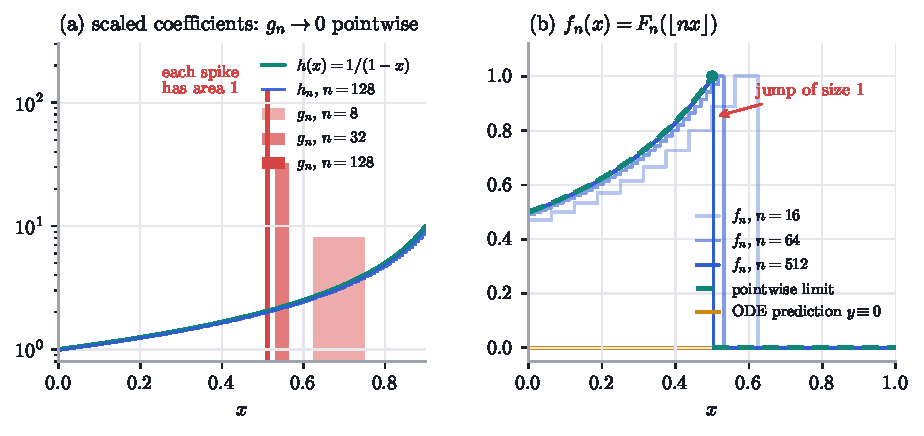
\includegraphics[width=\linewidth]{../figures/paper/fig1_counterexample.pdf}
\caption{The counterexample of \cref{thm:ce}. (a) The scaled forcing $g_n$ is a spike of
height $n$ and area $1$ that converges to $0$ at every point; $h_n$ converges to $1/(1-x)$.
(b) The recursion $f_n$ converges to $\frac{1}{2(1-x)}\1_{x\le1/2}$, not to the solution
$y\equiv0$ selected by the limiting equation.}\label{fig:ce}
\end{figure}

%=====================================================================
\section{The measure-valued limit theorem}\label{sec:measure}
%=====================================================================

We work with finite positive Borel measures on $[0,b]$ and weak convergence: $\nu_n\weak\nu$
means $\int\varphi\dd\nu_n\to\int\varphi\dd\nu$ for every $\varphi\in C[0,b]$. We use two
standard facts \cite[Thm.~2.1 and Thm.~2.7]{Bil99}, valid for finite positive measures since
$\nu_n([0,b])\to\nu([0,b])$ (if $\nu([0,b])>0$ normalise; if $\nu([0,b])=0$ both are trivial):
\begin{enumerate}[label=(W\arabic*),itemsep=1pt]
\item\label{W1} $\limsup_n\nu_n(C)\le\nu(C)$ for every closed $C\subset[0,b]$;
\item\label{W2} $\int\psi\dd\nu_n\to\int\psi\dd\nu$ for every bounded Borel $\psi$ whose set of
discontinuity points is $\nu$-null.
\end{enumerate}

\begin{theorem}[Measure-valued limit]\label{thm:main}
Assume \eqref{eq:Kn}, \eqref{eq:recK} and
\begin{enumerate}[label=\textup{(A\arabic*)},itemsep=1pt]
\item\label{A1} $h\in C[0,b]$ and $\max_{0\le k<K_n}|h_n(k/n)-h(k/n)|\to0$;
\item\label{A2} $G_n\ge0$ and $\nu_n\weak\nu$ for a finite positive Borel measure $\nu$ on $[0,b]$;
\item\label{A3} $\mu_n\to\Theta\in\R$.
\end{enumerate}
Define
\begin{equation}\label{eq:limit}
f(x)=\int_{[x,b]}\Phi(x,s)\dd\nu(s)+\Theta\,\Phi(x,b),\qquad x\in[0,b].
\end{equation}
Then $f_n(x_n)\to f(x)$ whenever $x_n\to x\in(0,b)$ and $\nu(\{x\})=0$. In particular
$f_n(x)\to f(x)$ at every $x\in(0,b)$ outside the at most countable set of atoms of $\nu$.
\end{theorem}

\begin{proof}
Fix $x$ and $x_n\to x$, and put $k=k(n)=\fl{nx_n}$, so $k/n\to x$; for large $n$,
$k<K_n$ because $K_n/n\to b>x$. By \cref{lem:duhamel},
\[
f_n(x_n)=F_n(k)=\sum_{m=k}^{K_n-1}G_n(m)P_n(k,m)+\mu_nP_n(k,K_n).
\]
\emph{Step 1 (propagators).} Let $L=\max_{[0,b]}|h|\cdot\max_{[0,b]^2}\Phi$, a Lipschitz constant of
$\Phi$ in its first variable. By \cref{lem:prop} and $G_n\ge0$,
\[
\Bigl|\sum_{m=k}^{K_n-1}G_n(m)P_n(k,m)-\int_{[k/n,b]}\Phi(x,s)\dd\nu_n(s)\Bigr|
\le\nu_n([0,b])\bigl(\varepsilon_n+L\,|k/n-x|\bigr)\to0,
\]
since $\sup_n\nu_n([0,b])<\infty$ by \ref{A2} (test with $\varphi\equiv1$).

\emph{Step 2 (the moving left endpoint).} Given $\eta>0$, for large $n$ the symmetric difference of
$[k/n,b]$ and $[x,b]$ lies in $C_\eta=[x-\eta,x+\eta]\cap[0,b]$, so
\[
\Bigl|\int_{[k/n,b]}\Phi(x,s)\dd\nu_n(s)-\int_{[x,b]}\Phi(x,s)\dd\nu_n(s)\Bigr|
\le\|\Phi\|_\infty\,\nu_n(C_\eta).
\]
By \ref{W1}, $\limsup_n\nu_n(C_\eta)\le\nu(C_\eta)$, and $\nu(C_\eta)\downarrow\nu(\{x\})=0$ as
$\eta\downarrow0$.

\emph{Step 3 (the limit of the integral).} The function $\psi(s)=\1_{[x,b]}(s)\Phi(x,s)$ is bounded and
continuous except possibly at $s=x$, a $\nu$-null point. By \ref{W2},
$\int\psi\dd\nu_n\to\int\psi\dd\nu=\int_{[x,b]}\Phi(x,s)\dd\nu(s)$.

\emph{Step 4 (terminal term).} $|P_n(k,K_n)-\Phi(x,b)|\le\varepsilon_n+|\Phi(k/n,K_n/n)-\Phi(x,b)|\to0$
by continuity of $\Phi$, and $\mu_n\to\Theta$.

Combining the four steps gives $f_n(x_n)\to f(x)$.
\end{proof}

\begin{remark}[What is, and is not, assumed]\label{rem:assumptions}
(a) No hypothesis on the limiting differential equation is needed on $[0,b]$; the role of the
conjecture's terminal-value selection is taken over by \ref{A3}.
(b) Signed forcing is handled by linearity: $F_n$ depends linearly on $(G_n,\mu_n)$ for fixed $H_n$.
If $\nu_n^\pm=\sum_kG_n(k)^\pm\delta_{k/n}$ converge weakly to $\nu^\pm$, the conclusion of
\cref{thm:main} holds with $\nu:=\nu^+-\nu^-$ whenever $x_n\to x\in(0,b)$ and
$\nu^+(\{x\})=\nu^-(\{x\})=0$. The limits $\nu^\pm$ need not be the Jordan parts of $\nu$, and
$\nu(\{x\})=0$ alone does not suffice: with $H_n\equiv1$, $\mu_n=0$ and spikes $+1$ at
$\fl{n/2}$ and $-1$ at $\fl{n/2}-1$, one has $\nu=0$ but $f_n(\frac12)=1$ for all $n$.
(c) Since $F_n(k)$ depends only on coefficients with index $\ge k$, \ref{A1}--\ref{A2} are needed
only on $[a,b]$ for each $a>0$ (with $\nu_n$ restricted there and $\nu(\{a\})=0$). This allows $h$ to
be singular at $0$, as in secretary-type recursions where $H_n(k)=\frac{k}{k+1}$ gives $h=1/x$.
(d) Hypothesis \ref{A1} is genuinely stronger than pointwise convergence. A single exceptional
value of $H_n$ (for instance $H_n(j_n)=\frac12$, as in the corollary of \cite{Pri26}) acts as a
\emph{multiplicative} spike; a version of \cref{thm:main} in which $h\dd x$ is also replaced by a
measure, and the propagator by a product integral, should hold but is not pursued here.
\end{remark}

%=====================================================================
\section{Consequences}\label{sec:consequences}
%=====================================================================

\begin{proposition}[Structure of the limit]\label{prop:structure}
Let $f$ be given by \eqref{eq:limit}, where $\nu$ may be any finite signed Borel measure on $[0,b]$.
Then:
\begin{enumerate}[label=\textup{(\roman*)},itemsep=1pt]
\item \emph{(semigroup form of $\mathrm{d}f=hf\dd x-\mathrm{d}\nu$)} for $0\le x<y\le b$,
\[f(x)=\Phi(x,y)\,f(y)+\int_{[x,y)}\Phi(x,s)\dd\nu(s);\]
\item \emph{(jumps)} $f$ is left-continuous on $(0,b]$ and has right limits, with
\[f(c^-)-f(c^+)=\nu(\{c\})\qquad(0<c<b);\]
\item \emph{(classical case)} if $\nu=g\dd s$ with $g\in C[0,b]$, then $f\in C^1[0,b]$ is the
unique solution of $y'=-g+hy$ with $y(b)=\Theta$.
\end{enumerate}
\end{proposition}

\begin{proof}
(i) Split $[x,b]=[x,y)\cup[y,b]$ and use $\Phi(x,s)=\Phi(x,y)\Phi(y,s)$.
(ii) As $y\uparrow x$, $|\nu|([y,x))\to0$ and $\Phi$ is uniformly continuous, so $f(y)\to f(x)$.
As $y\downarrow c$, $[y,b]\uparrow(c,b]$, so by dominated convergence (with respect to $|\nu|$)
$f(y)\to\int_{(c,b]}\Phi(c,s)\dd\nu(s)+\Theta\Phi(c,b)=f(c)-\nu(\{c\})$, using $\Phi(c,c)=1$.
(iii) Differentiate
$f(x)=\int_x^b\Phi(x,s)g(s)\dd s+\Theta\Phi(x,b)$ using $\partial_x\Phi=h\Phi$:
$f'(x)=-g(x)+h(x)f(x)$, and $f(b)=\Theta$. Uniqueness is standard for linear equations with
continuous coefficients.
\end{proof}

\begin{corollary}[Convergence under uniform integrability]\label{cor:ui}
Assume \eqref{eq:Kn}, \ref{A1}, \ref{A3}, $G_n\ge0$, and that $g_n\to g$ in $L^1(0,b)$ for some
$g\in C[0,b]$ (here $g_n:=0$ on $[K_n/n,b]$). Then $f_n(x)\to y(x)$ for \emph{every}
$x\in(0,b)$, where $y$ is the $C^1$ solution of $y'=-g+hy$, $y(b)=\Theta$. By Vitali's theorem
the $L^1$ hypothesis holds, for instance, if $g_n\to g$ almost everywhere and $\{g_n\}$ is
uniformly integrable, e.g.\ dominated by an integrable function.
\end{corollary}

\begin{proof}
For $\varphi\in C[0,b]$,
\[
\Bigl|\int\varphi\dd\nu_n-\int\varphi\, g_n\Bigr|
=\Bigl|\sum_mG_n(m)\Bigl(\varphi(\tfrac mn)-n\int_{m/n}^{(m+1)/n}\varphi\Bigr)\Bigr|
\le\omega_\varphi(1/n)\,\|g_n\|_{L^1}\to0,
\]
and $\int\varphi g_n\to\int\varphi g$. Hence $\nu_n\weak g\dd s$, which has no atoms; apply
\cref{thm:main} and \cref{prop:structure}(iii).
\end{proof}

\Cref{cor:ui} identifies the limit up to its terminal value: $\Theta=\lim_nF_n(K_n)$ is an input,
through \ref{A3}, not the value singled out by the endpoint hypothesis of the conjecture. When
$h$ and $g$ are continuous on $[0,1]$ every terminal value is admissible, so the conjecture's
hypothesis concerns singular $h$, where one must work on $[0,b]$ with $b<1$; relating
$\lim_nF_n(\fl{nb})$ to the selected value is the endpoint question of \cref{sec:discussion}.

In the counterexample, $\int g_n=1$ while $g_n\to0$ pointwise, so $\{g_n\}$ is not uniformly
integrable: all of its mass concentrates on a single interval of length $1/n$. Uniform
integrability is exactly the property that a pointwise check cannot see.
\Cref{fig:smooth}(b) shows a practical diagnostic: the largest mass of $\nu_n$ in a window of
half-width $\delta$ stays equal to $1$ for the spike, but decays like $\delta$ for smooth forcing.

\begin{corollary}[Fixed versus moving spikes]\label{cor:spikes}
Assume \eqref{eq:Kn}, let $H_n$ satisfy \ref{A1}, $\mu_n=0$, and let $G_n$ be a unit spike at an
index $j(n)<K_n$ with $j(n)/n\to c\in[0,b]$. If $c\in(0,b)$, then $f_n(x)\to\Phi(x,c)\1_{x<c}$ for
every $x\in(0,b)\setminus\{c\}$: the limit jumps by $1$ at $c$. If $c=b$, then
$f_n(x)\to\Phi(x,b)$ on $(0,b)$. If $c=0$, which includes a fixed index and $j(n)=\fl{\sqrt n}$,
then $f_n\to0$ on $(0,b)$: the spike washes out.
\end{corollary}

\begin{proof}
$\nu_n=\delta_{j(n)/n}\weak\delta_c$; apply \cref{thm:main}. For $c=0$ the atom lies outside
$[x,b]$ for every $x>0$.
\end{proof}

\begin{example}[The counterexample, recovered]\label{ex:recover}
Fix $b\in(\frac12,1)$ and $K_n=\fl{nb}$. For large $n$, $K_n>j_n$, so the recurrence on
$\{0,\dots,K_n\}$ has terminal value $\mu_n=F_n(K_n)=0$. For $k\le nb$,
$|h_n(k/n)-h(k/n)|=\frac{n}{(n-k)(n-k+1)}\le\frac{1}{n(1-b)^2}$, so \ref{A1} holds with
$h(x)=1/(1-x)$, and $\nu_n=\delta_{j_n/n}\weak\delta_{1/2}$. Here
$\Phi(x,s)=\frac{1-s}{1-x}$, and \cref{cor:spikes} gives $f(x)=\frac{1}{2(1-x)}$ for $x<\frac12$
and $f(x)=0$ for $\frac12<x<b$, which is \cref{thm:ce}(iv) for $x\in(0,b)\setminus\{\frac12\}$,
hence, $b$ being arbitrary, on $(0,1)\setminus\{\frac12\}$. The same computation with the spike at
$\fl{n/3}+1$ predicts $f_n(\frac14)\to\Phi(\frac14,\frac13)=\frac89$, and a spike at a fixed index
predicts $f_n(\frac14)\to0$ (\cref{fig:rates}(b)).
\end{example}

%=====================================================================
\section{Numerical experiments}\label{sec:numerics}
%=====================================================================

All numbers and figures are produced by a single Python script (\texttt{experiments.py}, provided
with the project files) using double precision, except where exact rational arithmetic is stated.

\paragraph{E1. Exact check of the closed form.} For every $4\le n\le\NexactMax$ we computed
$F_n$ from \eqref{eq:rec} in exact rational arithmetic and compared it with
\cref{thm:ce}; all values agree, lie in $[0,1]$, and $0<H_n<1$.

\paragraph{E2. Rate for the counterexample.} On $[0.05,0.45]\cup[0.55,0.95]$ the error
$\sup|f_n-f|$ decays with fitted slope $\SlopeCE$ in $\log n$ (least squares over $n\ge128$;
smaller $n$ are pre-asymptotic, \cref{fig:rates}(a)), reaching
$\ErrCEmax$ at $n=\NmaxCE$, where $f_n(\frac14)=\FquarterLast$.

\paragraph{E3. A generic test of \cref{thm:main}.} We took $h(x)=1+0.6\sin 2\pi x$,
perturbed it as $h_n(k/n)=h(k/n)+n^{-1/2}\sin(37k)$ (so $\delta_n\asymp n^{-1/2}$), smooth
forcing $g(x)=1+2x(1-x)$ discretised as $G_n(k)=g(k/n)/n$, two moving spikes of masses $0.8$ and
$0.5$ at indices $\fl{0.3n}+1$ and $\fl{0.7n}+1$, and $\mu_n=\Theta=0.4$. Away from the atoms
($|x-c|>0.02$) the error against \eqref{eq:limit} decays with slope $\SlopeGen$ (fitted over
$n\ge256$; the oscillating
perturbation averages out in the sums of \cref{lem:prop}), while the solution of the
differential equation built from the pointwise limits $g,h$ is off by up to $\GapGen$
(\cref{fig:general}).

\paragraph{E4. Smoothing the spike.} Spreading the unit mass uniformly over $|s-\frac12|<w/2$
makes $\nu$ absolutely continuous. \Cref{thm:main} applies (truncating at $b<1$ as in
\cref{ex:recover}); $\nu$ has no atoms, so convergence holds at every $x$, and the limits are
continuous and converge to the jump as $w\to0$ (\cref{fig:smooth}(a)). For $w=0.1$ and $n=4096$ the discrete
solution matches the predicted limit to $\SmoothErr$.

\paragraph{E5. Fixed versus moving spikes.} With $H_n$ from \cref{thm:ce}, spikes at
$\fl{n/2}+1$ and $\fl{n/3}+1$ give $f_n(\frac14)=\HalfLast$ and $\ThirdLast$ at $n=\NmaxFive$,
matching $\frac23$ and $\frac89$; spikes at index $3$ or $\fl{\sqrt n}$ give $\FixedLast$
(\cref{fig:rates}(b)). The last two values are exact once the spike lies below $\fl{n/4}$, since
$\mu_n=0$; they illustrate \cref{cor:spikes} rather than test a rate.

\begin{figure}[t]
\centering
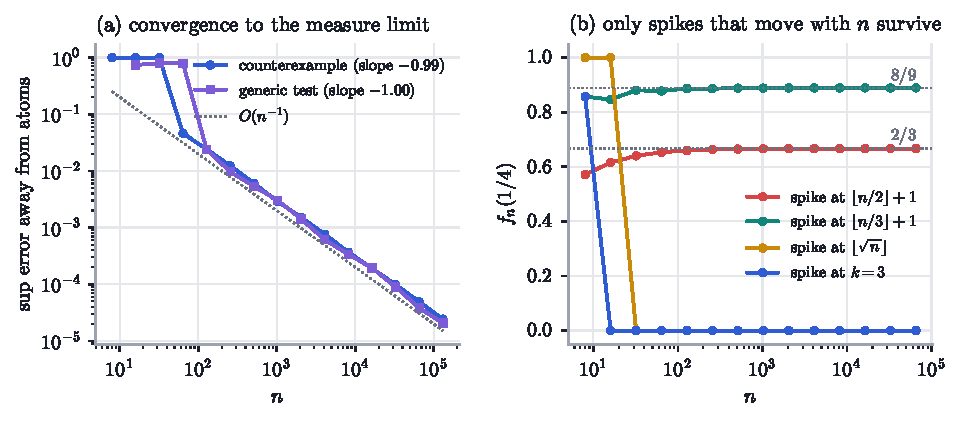
\includegraphics[width=\linewidth]{../figures/paper/fig2_rates_and_spikes.pdf}
\caption{(a) Sup-error to the limit \eqref{eq:limit} away from atoms, for the counterexample
(E2) and the generic test (E3). (b) $f_n(\frac14)$ for unit spikes at different indices (E5):
only spikes at a fixed relative position survive, with the limits predicted by \cref{cor:spikes}.}
\label{fig:rates}
\end{figure}

\begin{figure}[t]
\centering
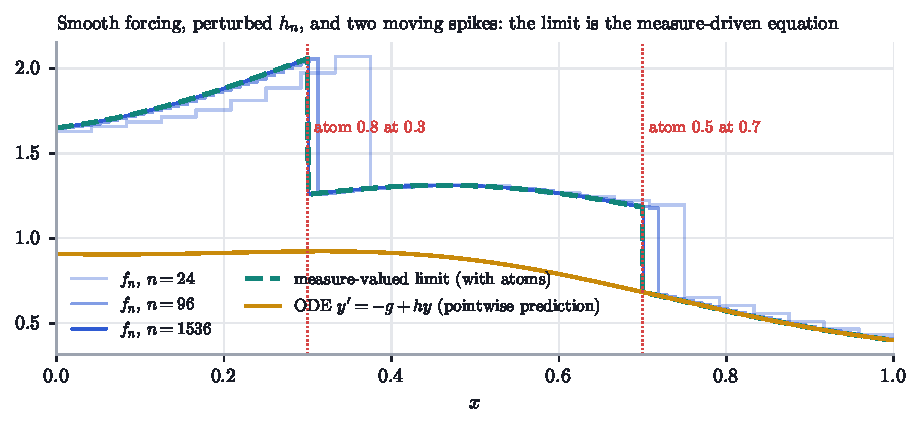
\includegraphics[width=\linewidth]{../figures/paper/fig3_general_theorem.pdf}
\caption{Experiment E3. With smooth forcing, a perturbed $h_n$ and two moving spikes, the recursion
converges to the measure-driven limit \eqref{eq:limit}, with jumps equal to the spike masses, and
not to the solution of the differential equation built from the pointwise limits.}
\label{fig:general}
\end{figure}

\begin{figure}[t]
\centering
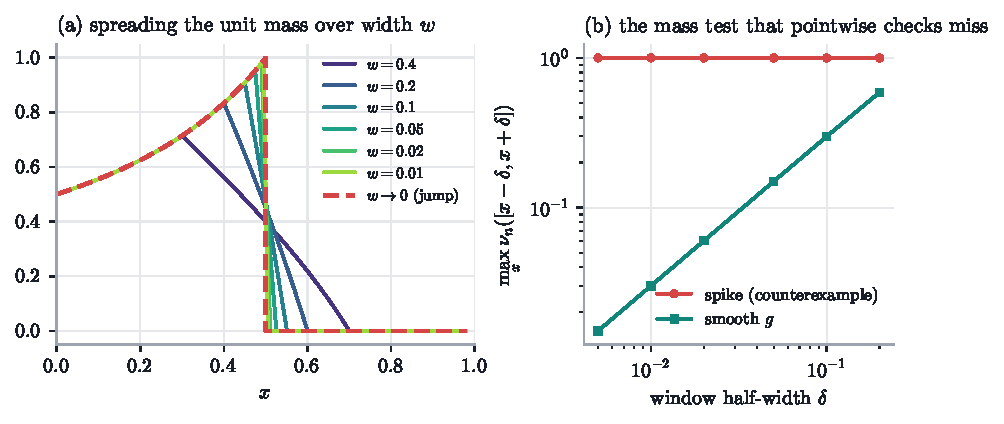
\includegraphics[width=\linewidth]{../figures/paper/fig4_smoothing_and_mass.pdf}
\caption{(a) Limits for a unit mass spread over width $w$ (E4), converging to the jump as $w\to0$.
(b) The window-mass diagnostic $\max_x\nu_n([x-\delta,x+\delta])$ at $n=4096$: it stays at $1$ for
the spike and decays linearly for smooth forcing.}
\label{fig:smooth}
\end{figure}

%=====================================================================
\section{Backpropagation through residual networks}\label{sec:sciml}
%=====================================================================

Residual networks $z_{k+1}=z_k+\frac1n v(z_k,\theta)$ are forward Euler discretisations of
$\dot z=v(z,\theta)$ on $[0,1]$ \cite{E17,HR18}, and neural ODEs \cite{CRBD18} train the
continuous model directly, computing gradients with the adjoint equation. That backpropagation
through a discretisation is a discrete adjoint consistent with the continuous one is classical in
optimal control and its neural-ODE incarnations \cite{Hag00,SS16,GKB19}. The deep-layer limit of
residual networks has been studied in a variational sense \cite{TvG23}, and trained weights need
not converge to a smooth function of depth \cite{CCRX21}. Here we point out that the
\emph{backward} pass is itself a recurrence of the form \eqref{eq:rec}, so that
\cref{thm:main} describes its continuous limit, including in a situation that a pointwise view
of the coefficients gets wrong.

Consider a scalar state (we expect the vector case, with matrix products, to be analogous),
$z_0$ given, parameters $\theta$, and a loss with terminal and intermediate terms,
\begin{equation}\label{eq:loss}
L_n(\theta)=\Psi(z_n)+\sum_{i=1}^r w_i\,\ell_i\bigl(z_{k_i(n)}\bigr),\qquad k_i(n)/n\to\tau_i\in(0,1),
\end{equation}
as in deep supervision or in training on a time series observed at intermediate times
\cite{RCD19}. Backpropagation computes $\lambda_k=\partial L_n/\partial z_k$ by
\begin{equation}\label{eq:backprop}
\lambda_n=\Psi'(z_n),\qquad
\lambda_k=\underbrace{\sum_i[k=k_i(n)]\,w_i\ell_i'(z_k)}_{G_n(k)}
+\underbrace{\Bigl(1+\tfrac1n\partial_zv(z_k,\theta)\Bigr)}_{H_n(k)}\lambda_{k+1},
\end{equation}
and $\nabla_\theta L_n=\frac1n\sum_{k=0}^{n-1}\lambda_{k+1}\,\partial_\theta v(z_k,\theta)$.
So $h_n(k/n)=-\partial_zv(z_k,\theta)$, and every intermediate loss is a spike of size $O(1)$ at
relative depth $\tau_i$.

\begin{proposition}[Adjoints jump at intermediate losses]\label{prop:adjoint}
Let $v$ be $C^2$ with bounded derivatives, $\Psi,\ell_i\in C^1$, let $z$ solve $\dot z=v(z,\theta)$,
$z(0)=z_0$, and put $\Phi(t,s)=\exp\int_t^s\partial_zv(z(r),\theta)\dd r$. Let $\lambda$ be the solution of
\[
\dot\lambda=-\partial_zv(z(t),\theta)\,\lambda\ \text{ on }(0,1)\setminus\{\tau_i\},\qquad
\lambda(1)=\Psi'(z(1)),\qquad \lambda(\tau_i^-)-\lambda(\tau_i^+)=w_i\,\ell_i'(z(\tau_i)),
\]
normalised to be left-continuous. Then $\lambda_{\fl{nt}}\to\lambda(t)$ for every
$t\in(0,1)\setminus\{\tau_i\}$, and
$\nabla_\theta L_n\to\int_0^1\lambda(t)\,\partial_\theta v(z(t),\theta)\dd t$.
In contrast, the continuous adjoint built from the pointwise limits of the coefficients in
\eqref{eq:backprop} (which exist for $t\notin\{\tau_i\}$, where $g_n(t)\to0$) has no jumps, and its
gradient differs from the limit by
\[
\sum_iw_i\,\ell_i'(z(\tau_i))\int_0^{\tau_i}\Phi(t,\tau_i)\,\partial_\theta v(z(t),\theta)\dd t,
\]
which is nonzero in general.
\end{proposition}

\begin{proof}
Euler's method converges, $\max_k|z_k-z(k/n)|=O(1/n)$ \cite{HNW93}, and $\partial_zv$ is Lipschitz,
so \ref{A1} holds with $h(t)=-\partial_zv(z(t),\theta)$, $b=1$, $K_n=n$, and $\Phi$ above is the
propagator \eqref{eq:Phi}. By linearity and \cref{lem:duhamel},
$\lambda_k=\Psi'(z_n)P_n(k,n)+\sum_i a_{i,n}P_n(k,k_i(n))\1_{k\le k_i(n)}$ with
$a_{i,n}=w_i\ell_i'(z_{k_i(n)})\to a_i:=w_i\ell_i'(z(\tau_i))$. Let $t_n\to t\notin\{\tau_i\}$ and
$k=\fl{nt_n}$. By \cref{lem:prop} and continuity of $\Phi$, $\Psi'(z_n)P_n(k,n)\to\Psi'(z(1))\Phi(t,1)$
and $a_{i,n}P_n(k,k_i(n))\to a_i\Phi(t,\tau_i)$, while $\1_{k\le k_i(n)}\to\1_{t<\tau_i}$ because
$k/n\to t\neq\tau_i$. Hence $\lambda_{\fl{nt_n}}\to\Psi'(z(1))\Phi(t,1)+\sum_ia_i\Phi(t,\tau_i)\1_{t<\tau_i}$,
which is the jump adjoint above (this is \eqref{eq:limit} with $\nu=\sum_ia_i\delta_{\tau_i}$, and the
argument needs no sign condition, even if several $\tau_i$ coincide). Writing the gradient as
$\int_0^1\lambda_{\fl{nt}+1}\,\partial_\theta v(z_{\fl{nt}},\theta)\dd t$, the integrand is bounded
uniformly in $n$ (by \cref{lem:prop}) and converges for all but finitely many $t$ (take $t_n=t+\frac1n$);
dominated convergence concludes. The last statement follows by subtracting the atomic part.
\end{proof}

The jump condition is the one used in practice when a neural ODE is trained on observations at
several times: the adjoint state is updated by the loss gradient at each observation time
\cite{CRBD18,RCD19}. \Cref{prop:adjoint} places it inside the framework of \cref{thm:main}: it is what
backpropagation through the discretised network converges to, whereas an adjoint obtained by
passing to the limit pointwise in the coefficients converges to a different gradient.

\paragraph{E6. Experiment.} We took $v(z,\alpha,\beta)=\tanh(\alpha z+\beta)$ with $\alpha=1.3$,
$\beta=0.4$, $z_0=0.5$, $\Psi(z)=\frac12(z-0.2)^2$, and one intermediate loss
$\frac12z_{\fl{n/2}}^2$ ($w_1=1$, $\tau_1=\frac12$). Backpropagation via \eqref{eq:backprop} agrees
with central finite differences to $\FDdiff$ at $n=64$. \Cref{tab:adjoint} and \cref{fig:adjoint}
compare $\partial L_n/\partial\alpha$ with the continuous gradients computed with the jump adjoint
($\GradJump$) and with the pointwise adjoint ($\GradNaive$): the discrete gradient converges to
the former with slope $\SlopeAdj$ (fitted over $n\ge64$), while the pointwise-adjoint gradient differs
from the limit by $\GradRelErr\%$, and from the discrete gradient by at least $0.0867$ at every depth
tested.

\begin{table}[t]
\centering
\begin{tabular}{rccc}
\toprule
depth $n$ & $\partial L_n/\partial\alpha$ & error vs.\ jump adjoint & error vs.\ pointwise adjoint\\
\midrule
\AdjointRows
\bottomrule
\end{tabular}
\caption{Experiment E6: parameter gradients of a residual network with one intermediate loss.}
\label{tab:adjoint}
\end{table}

\begin{figure}[t]
\centering
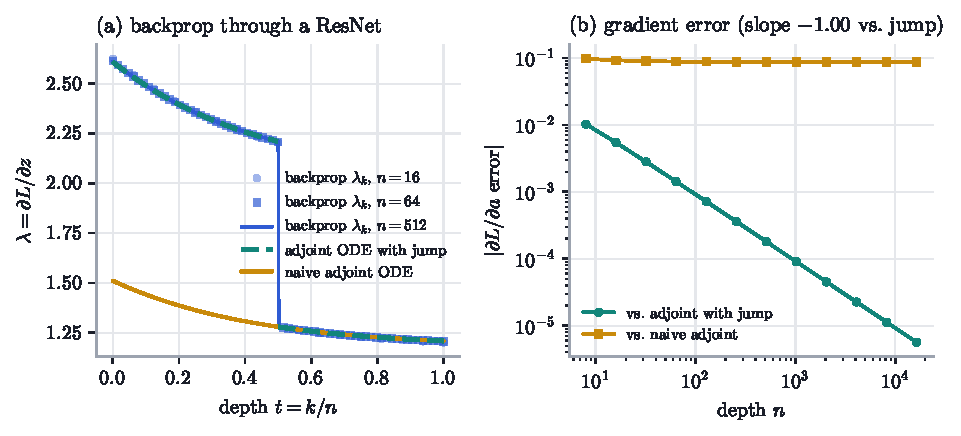
\includegraphics[width=\linewidth]{../figures/paper/fig5_resnet_adjoint.pdf}
\caption{Experiment E6. (a) The backpropagated adjoints $\lambda_k$ converge to the adjoint with a
jump at depth $\frac12$, not to the smooth adjoint obtained from the pointwise limits.
(b) Error of the parameter gradient against both continuous candidates.}
\label{fig:adjoint}
\end{figure}

\paragraph{Beyond residual networks.} The same linear structure appears whenever a quantity is
computed by backward induction with impulsive inputs: policy evaluation in continuous-time
reinforcement learning \cite{Doy00} with rewards concentrated at particular times, reserves with
lump-sum payments, or present values with discrete dividends. Analogous jump conditions are
classical in these settings, and measure differential equations have a classical theory \cite{DS72};
\cref{thm:main} is the scalar linear discrete-to-continuum statement, and suggests a simple
diagnostic: check whether the forcing \emph{measures} converge, and where their atoms are, rather
than whether the coefficients converge pointwise.

%=====================================================================
\section{Discussion and open questions}\label{sec:discussion}
%=====================================================================

\Cref{thm:main} replaces the pointwise hypothesis on $g_n$ by weak convergence of the forcing
measures, which is the natural hypothesis (the counterexample) and is sufficient (the theorem), and
it identifies the limit as the solution of a measure-driven equation. Several questions remain.

\begin{enumerate}[leftmargin=2em,itemsep=2pt]
\item \emph{Multiplicative spikes.} Replace \ref{A1} by convergence of the measures $h_n\dd x$
(allowing atoms in $\log H_n$) and the propagator by a product integral, so that the corollary of
\cite{Pri26} with $H_n(j_n)=\frac12$ is covered.
\item \emph{Endpoint singularities.} When $h$ is not integrable at $b=1$, as for $h=1/(1-x)$,
we restricted to $[0,b]$ with $b<1$. A statement on $(0,1)$ requires controlling $F_n$ near the
terminal index; this is the third follow-up question of \cite{Pri26} (endpoint selection).
\item \emph{Rates.} The experiments show $O(1/n)$ in typical cases. We expect a quantitative version
of \cref{thm:main} in terms of $\delta_n$, $\omega_h$ and a Wasserstein-type distance between $\nu_n$
and $\nu$ (the fourth follow-up question); since $\1_{[x,b]}$ is not Lipschitz, it also needs local
mass bounds for $\nu$ near $x$.
\item \emph{Signed forcing without splitting.} \Cref{rem:assumptions}(b) requires the positive and
negative parts to converge separately; mass that cancels at a common location can behave differently,
as the example given there shows.
\end{enumerate}

\paragraph{Acknowledgements.} I thank the Principia Math team for the platform and for the solution and
Lean formalisation \cite{Pri26,PriLean} on which \cref{sec:counterexample} is based.

\begin{thebibliography}{99}\small
\bibitem{BFGOR23} L.~Bay\'on, P.~Fortuny Ayuso, J.~M.~Grau, A.~M.~Oller-Marc\'en, M.~M.~Ruiz,
\emph{A new method for computing asymptotic results in optimal stopping problems},
Bull.\ Malays.\ Math.\ Sci.\ Soc.\ \textbf{46} (2023), article 46.
\href{https://doi.org/10.1007/s40840-022-01436-4}{doi:10.1007/s40840-022-01436-4};
preprint \href{https://arxiv.org/abs/2205.08495}{arXiv:2205.08495}.
\bibitem{Bil99} P.~Billingsley, \emph{Convergence of Probability Measures}, 2nd ed., Wiley, 1999.
\bibitem{CRBD18} R.~T.~Q.~Chen, Y.~Rubanova, J.~Bettencourt, D.~Duvenaud, \emph{Neural ordinary
differential equations}, Advances in Neural Information Processing Systems 31 (2018).
\bibitem{CCRX21} A.-S.~Cohen, R.~Cont, A.~Rossier, R.~Xu, \emph{Scaling properties of deep residual
networks}, Proceedings of the 38th International Conference on Machine Learning, PMLR 139 (2021).
\bibitem{DS72} P.~C.~Das, R.~R.~Sharma, \emph{Existence and stability of measure differential
equations}, Czechoslovak Math.\ J.\ \textbf{22} (1972), 145--158.
\href{https://doi.org/10.21136/CMJ.1972.101082}{doi:10.21136/CMJ.1972.101082}.
\bibitem{Doy00} K.~Doya, \emph{Reinforcement learning in continuous time and space},
Neural Computation \textbf{12} (2000), 219--245.
\bibitem{E17} W.~E, \emph{A proposal on machine learning via dynamical systems},
Commun.\ Math.\ Stat.\ \textbf{5} (2017), 1--11.
\bibitem{Fer89} T.~S.~Ferguson, \emph{Who solved the secretary problem?}, Statist.\ Sci.\
\textbf{4} (1989), 282--296.
\bibitem{GM66} J.~P.~Gilbert, F.~Mosteller, \emph{Recognizing the maximum of a sequence},
J.\ Amer.\ Statist.\ Assoc.\ \textbf{61} (1966), 35--73.
\bibitem{GKB19} A.~Gholami, K.~Keutzer, G.~Biros, \emph{ANODE: unconditionally accurate memory-efficient
gradients for neural ODEs}, Proceedings of the 28th International Joint Conference on Artificial
Intelligence (IJCAI 2019).
\bibitem{Hag00} W.~W.~Hager, \emph{Runge--Kutta methods in optimal control and the transformed adjoint
system}, Numer.\ Math.\ \textbf{87} (2000), 247--282.
\bibitem{HR18} E.~Haber, L.~Ruthotto, \emph{Stable architectures for deep neural networks},
Inverse Problems \textbf{34} (2018), 014004.
\bibitem{HNW93} E.~Hairer, S.~P.~N{\o}rsett, G.~Wanner, \emph{Solving Ordinary Differential
Equations I: Nonstiff Problems}, 2nd ed., Springer, 1993.
\bibitem{Pri26} Principia Math in Progress, \emph{A bounded counterexample to pointwise convergence
for recurrence-defined functions}, solution to MathDB problem 354674, Principia, September 2026.
\url{https://mathdb.com/p/354674}.
\bibitem{MST19} G.~A.~Monteiro, A.~Slav\'ik, M.~Tvrd\'y, \emph{Kurzweil--Stieltjes Integral: Theory and
Applications}, World Scientific, 2019.
\bibitem{PriLean} Principia Math, Lean~4 formalisation \texttt{Problem354674.lean},
\url{https://github.com/PrincipiaMathOrg/math-solutions/blob/main/mathdb/Principia/MathDB/Problem354674.lean}.
\bibitem{Rav24} A.~Ravsky, answers on MathOverflow question 463221 and Mathematics Stack Exchange
question 4862107, February 2024.
\bibitem{Sch92} \v{S}.~Schwabik, \emph{Generalized Ordinary Differential Equations}, World Scientific, 1992.
\bibitem{SS16} J.~M.~Sanz-Serna, \emph{Symplectic Runge--Kutta schemes for adjoint equations, automatic
differentiation, optimal control, and more}, SIAM Rev.\ \textbf{58} (2016), 3--33.
\bibitem{RCD19} Y.~Rubanova, R.~T.~Q.~Chen, D.~Duvenaud, \emph{Latent ordinary differential equations
for irregularly-sampled time series}, Advances in Neural Information Processing Systems 32 (2019).
\bibitem{TvG23} M.~Thorpe, Y.~van Gennip, \emph{Deep limits of residual neural networks},
Res.\ Math.\ Sci.\ \textbf{10} (2023), article 6.
\href{https://doi.org/10.1007/s40687-022-00370-y}{doi:10.1007/s40687-022-00370-y}.
\end{thebibliography}

\end{document}
